\subsection{Motivations \& Architecture}

% * * * * * * NEW FRAME * * * * * * %
\begin{frame}{New requirements: federation}
    \begin{center}
        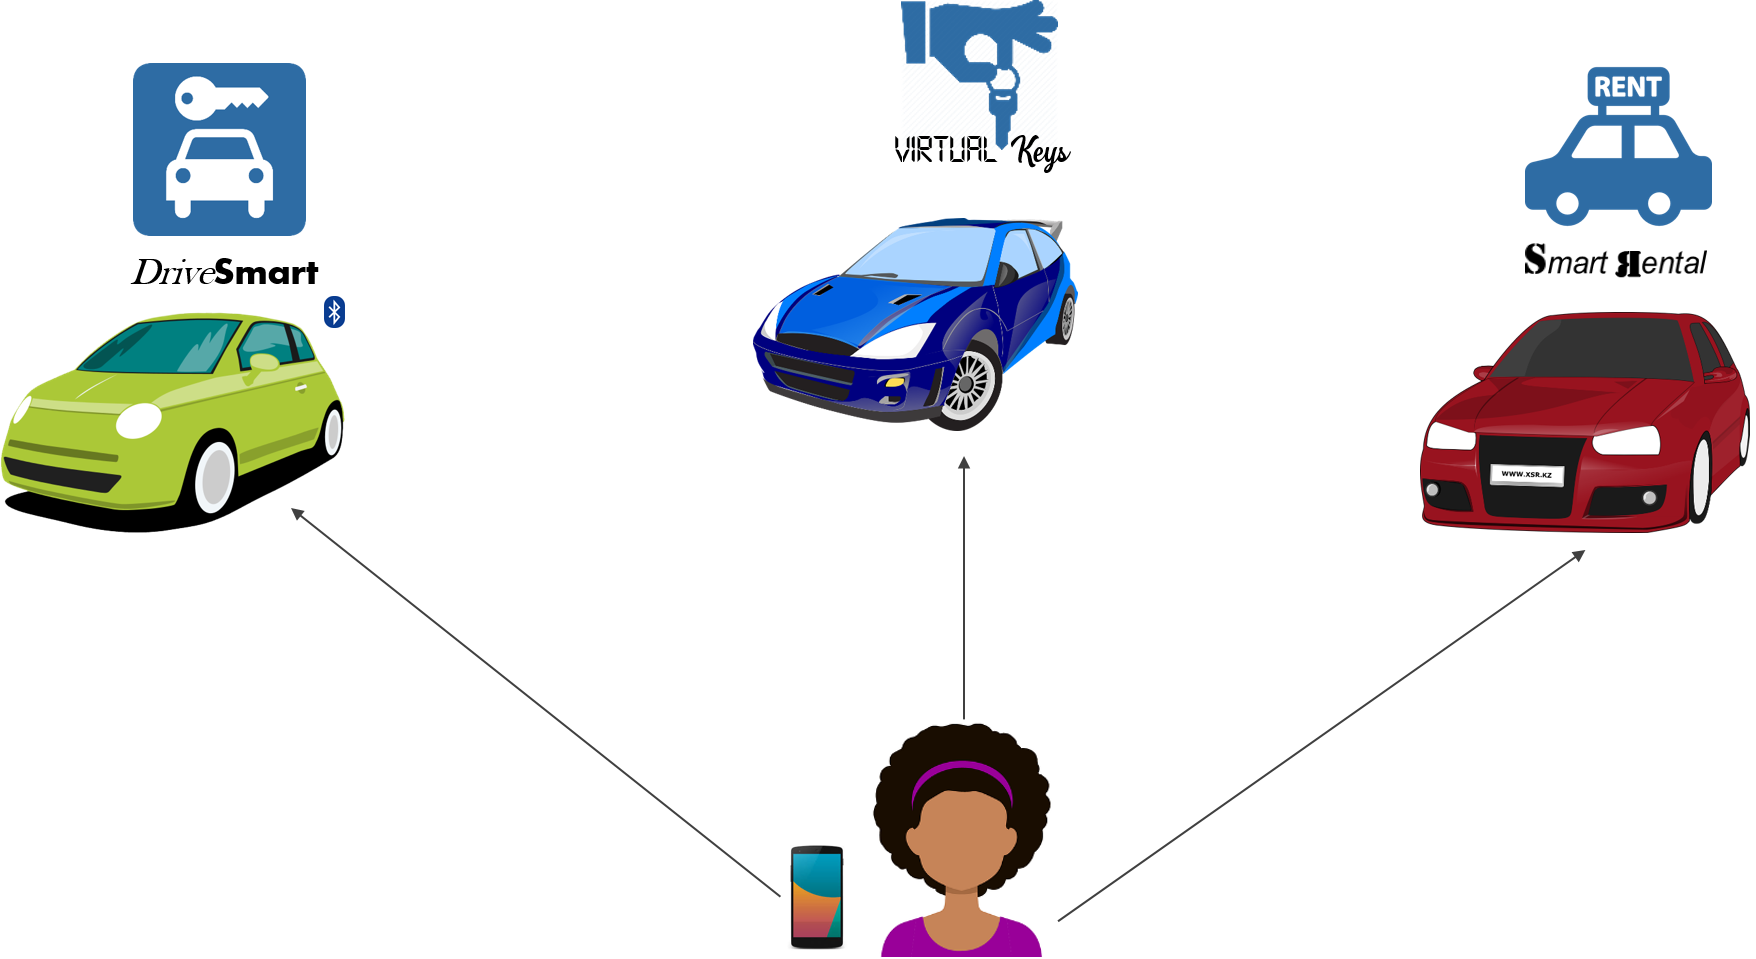
\includegraphics[scale=0.33]{Figures/ex_MAAC-B.png}
    \end{center}
    
    \begin{multicols}{2}
        \begin{itemize}
            \item Interoperability
            \item Dynamic users
            \item User-centric
            \item Scalability
            \item Ease of management
            \item Local access
        \end{itemize}
    \end{multicols}
\end{frame}

% * * * * * * NEW FRAME * * * * * * %
\begin{frame}{Setting up the system}
    \begin{center}
        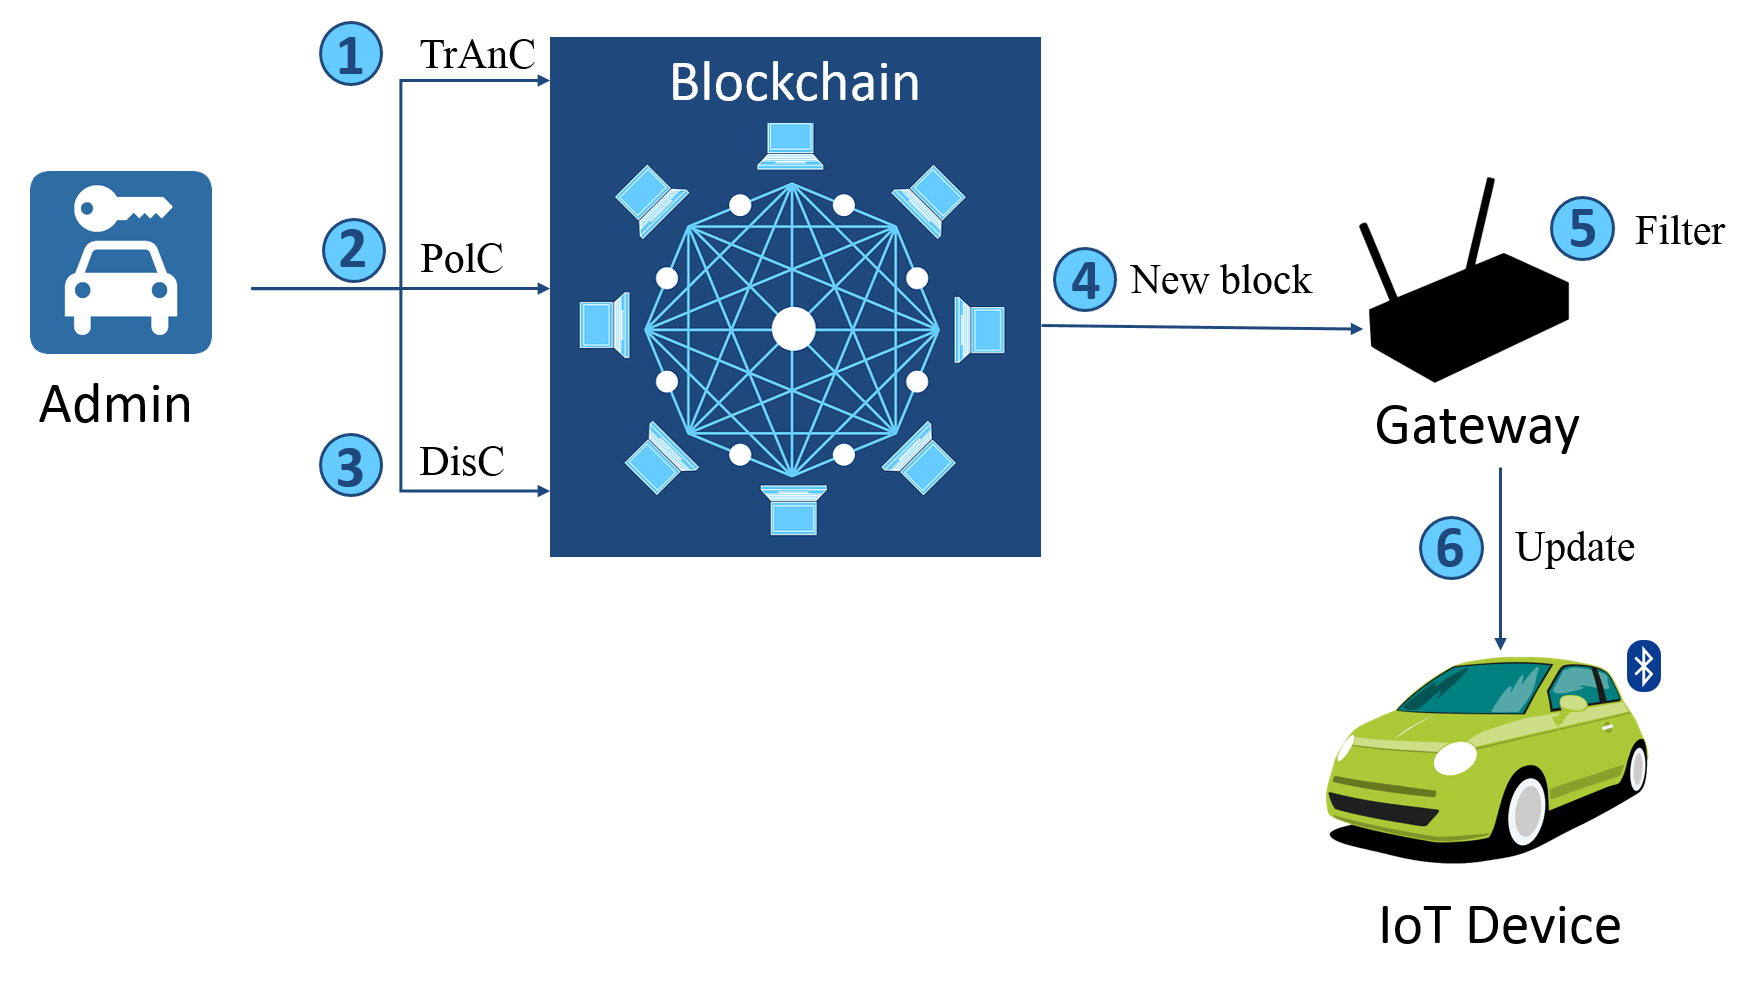
\includegraphics[scale=0.36]{Figures/MAAC-B_bootstrap.png}
    \end{center}
\end{frame}

% * * * * * * NEW FRAME * * * * * * %
\begin{frame}{Access control overview}
    \begin{center}
        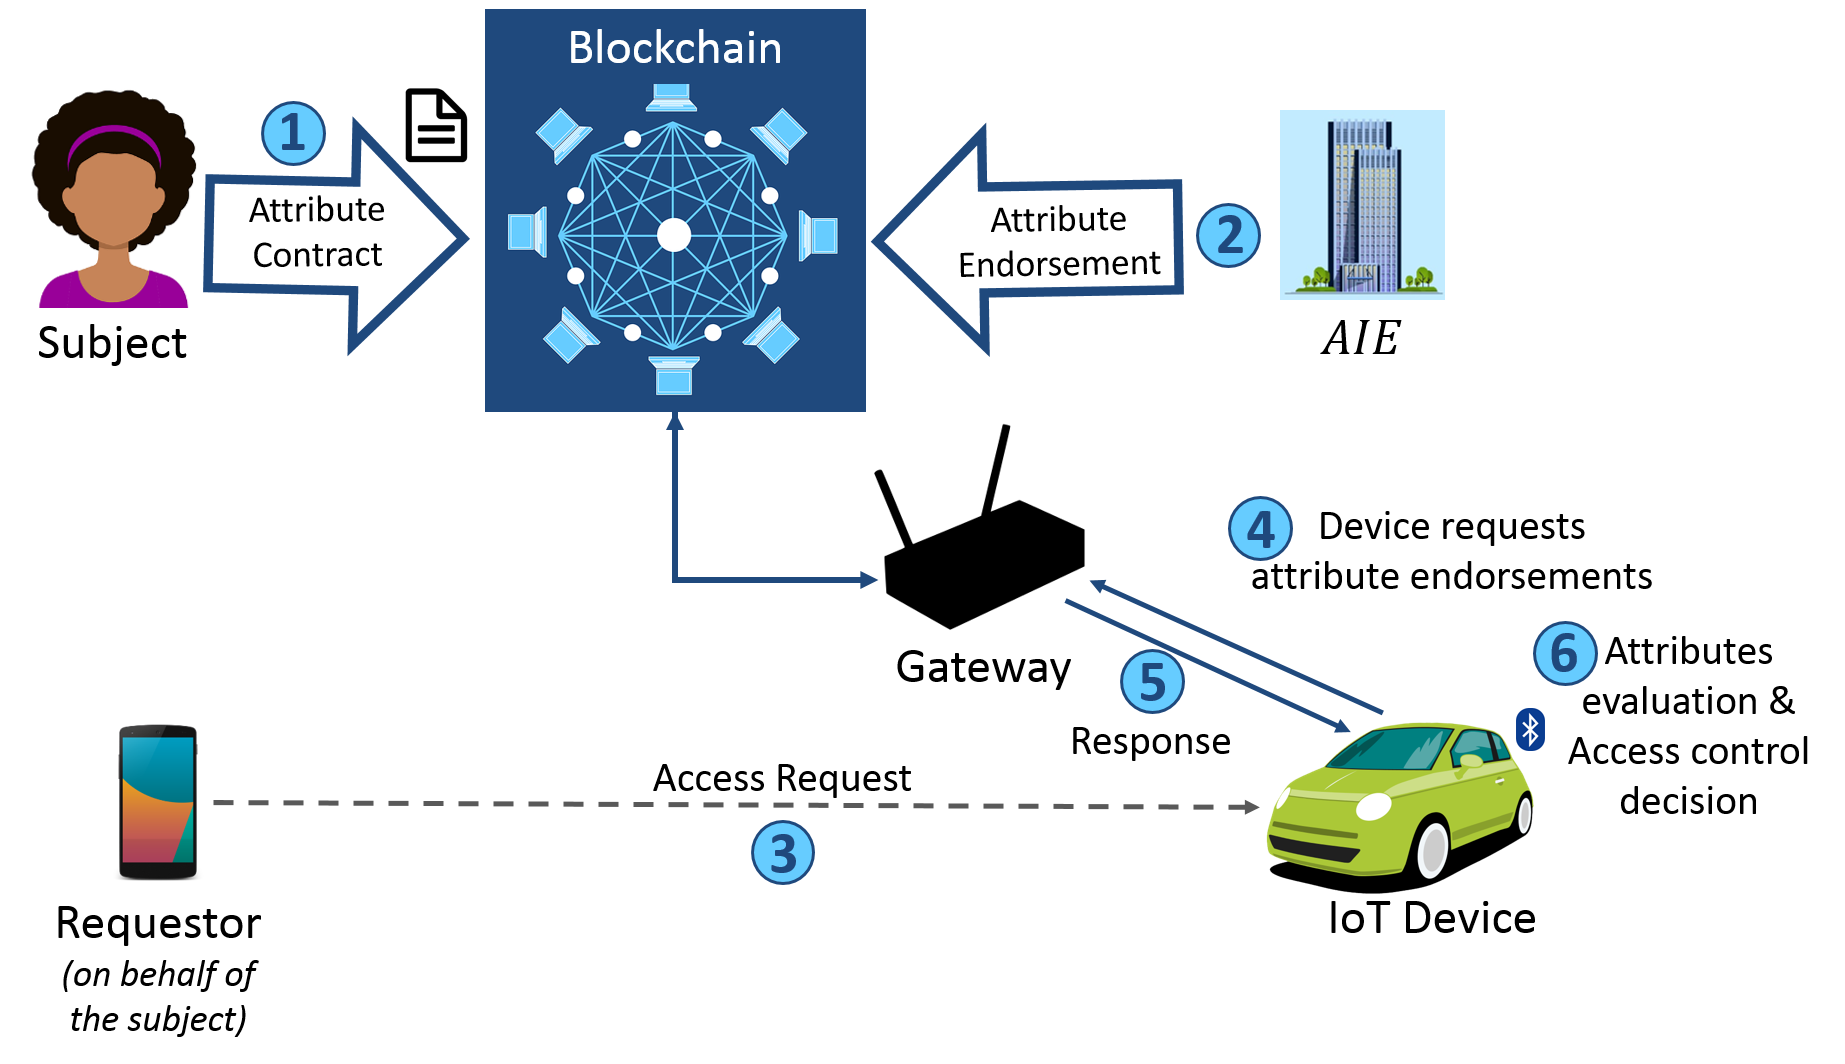
\includegraphics[scale=0.36]{Figures/MAAC-B_AC_high_level.png}
    \end{center}
\end{frame}


\subsection{Blockchain services}

% * * * * * * NEW FRAME * * * * * * %
\begin{frame}{Trust Anchor Service}
    \begin{center}
        \only<1>{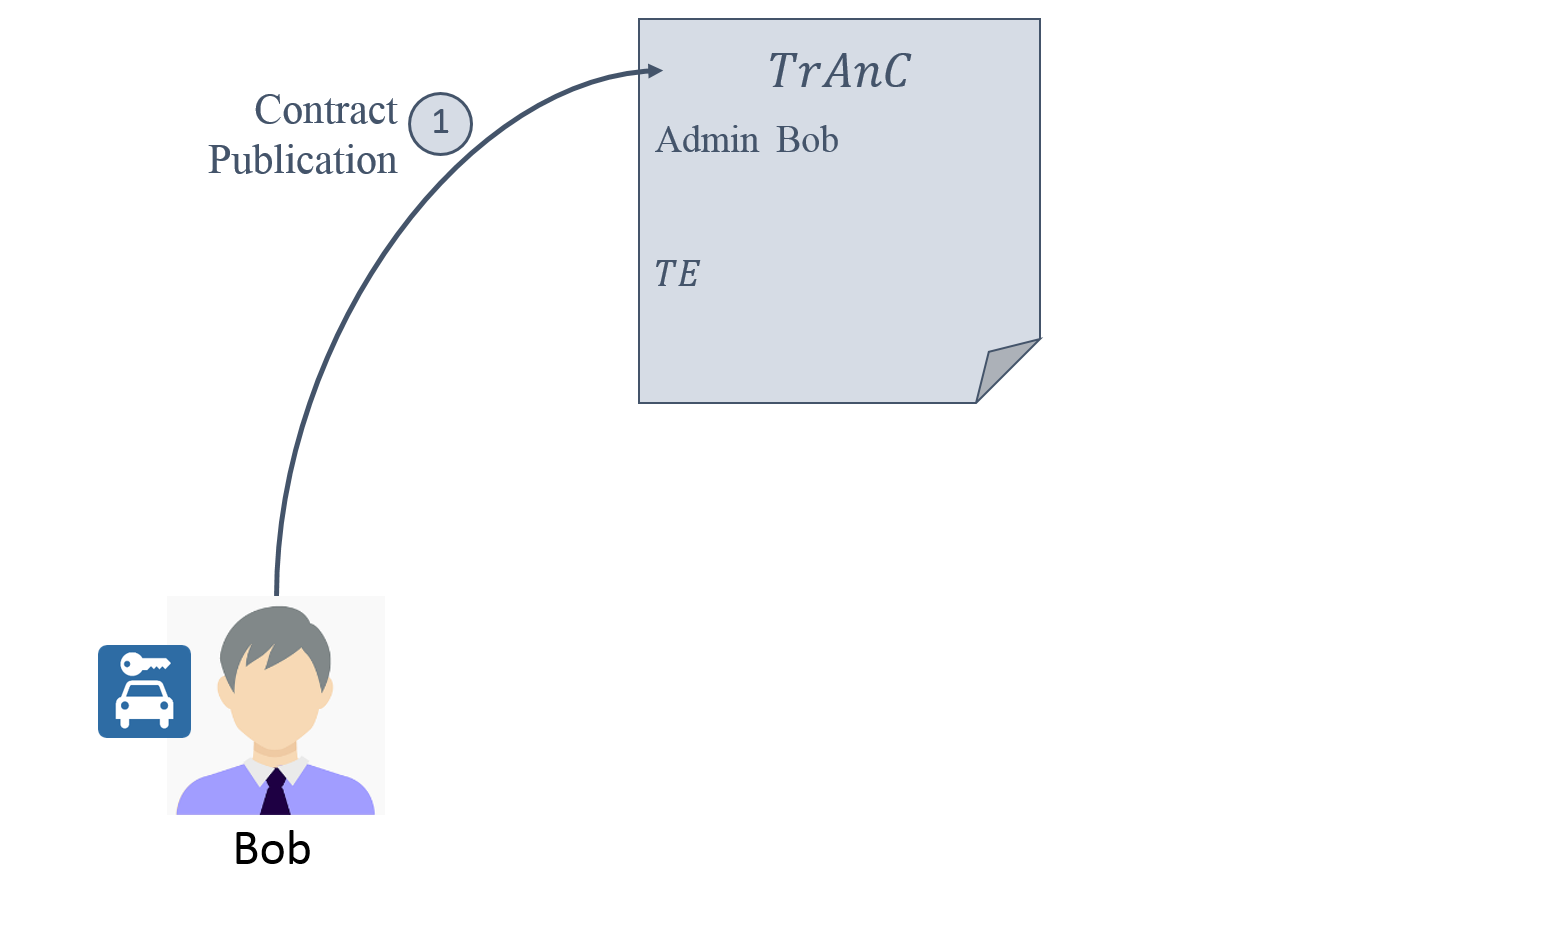
\includegraphics[scale=0.4]{Figures/TrAnC_1.png}}
        \only<2>{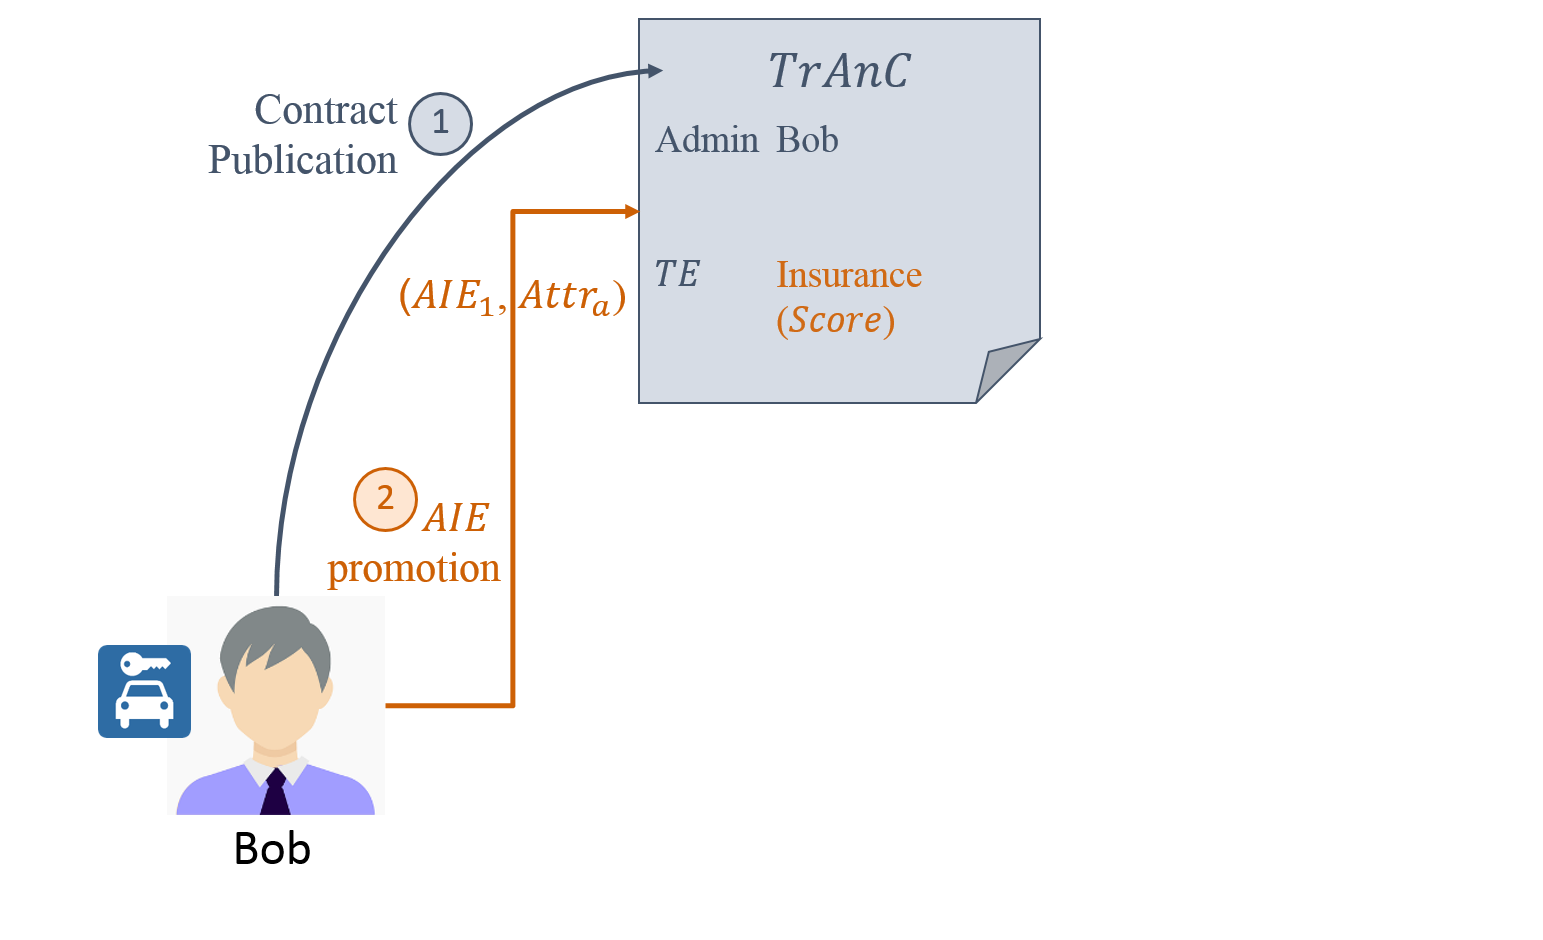
\includegraphics[scale=0.4]{Figures/TrAnC_2.png}}        
        \only<3>{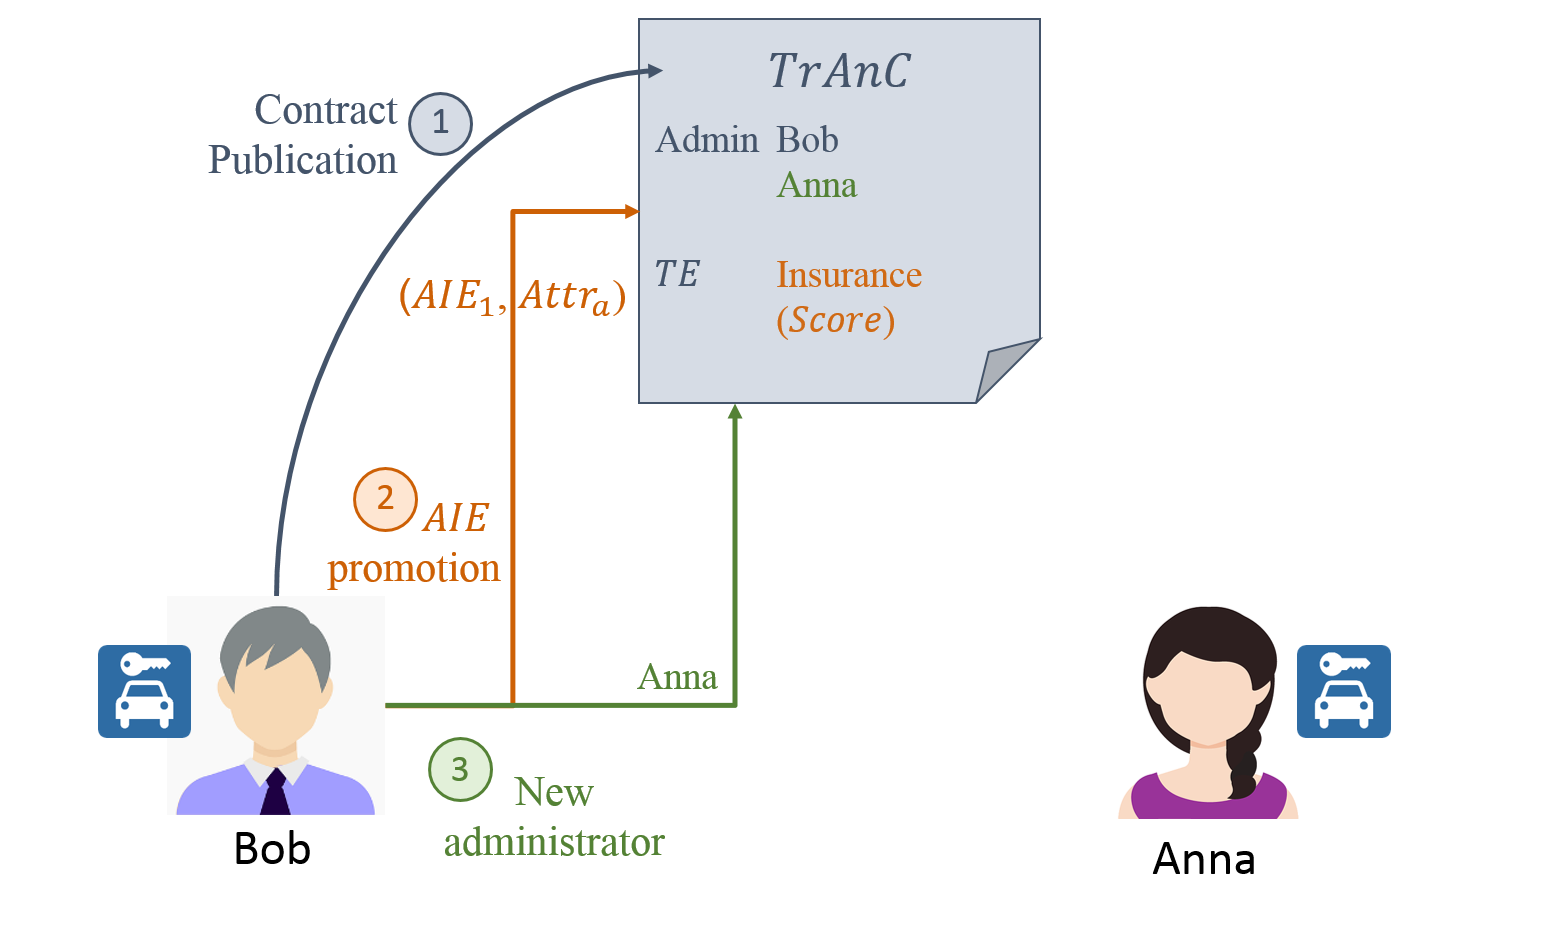
\includegraphics[scale=0.4]{Figures/TrAnC_3.png}}
        \only<4>{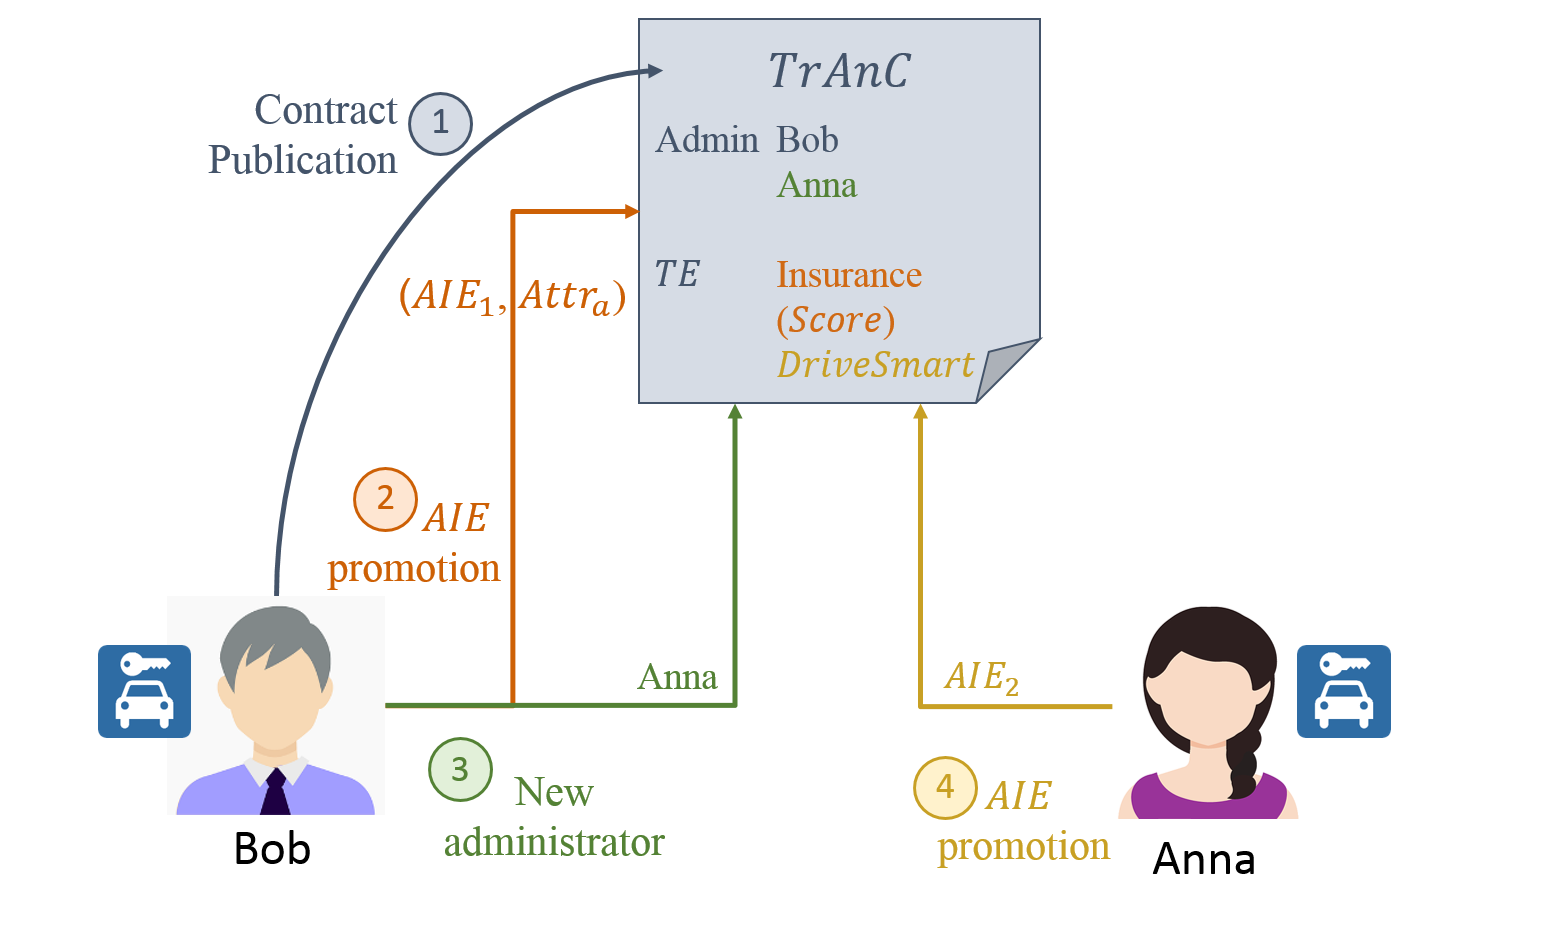
\includegraphics[scale=0.4]{Figures/TrAnC_4.png}}
        \only<5>{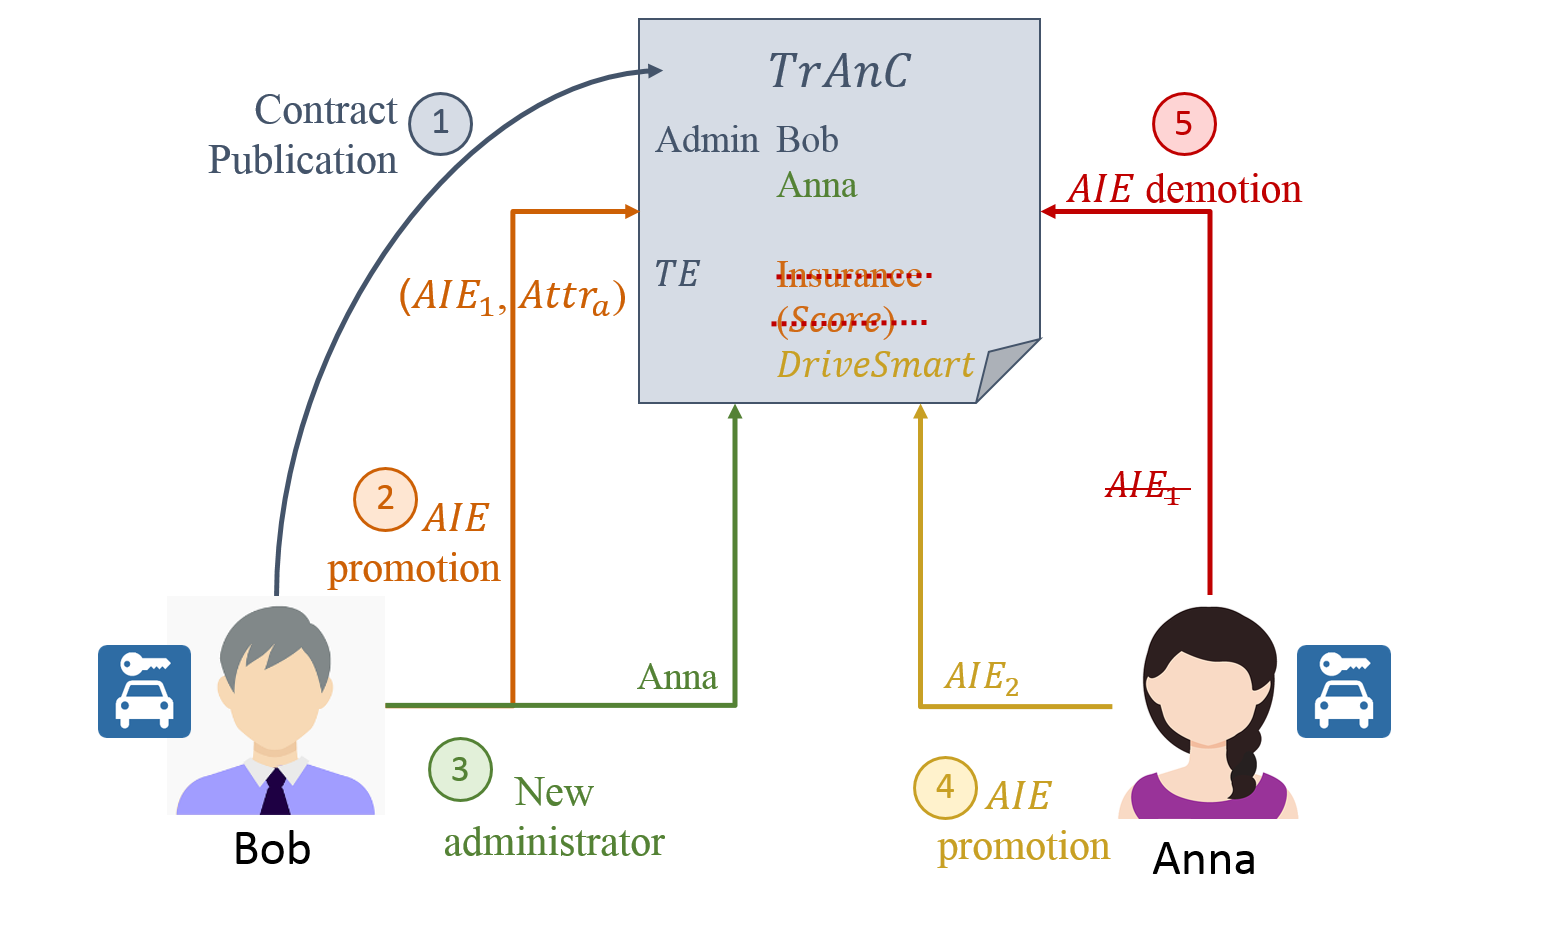
\includegraphics[scale=0.4]{Figures/TrAnC_5.png}}
    \end{center}
\end{frame}

% * * * * * * NEW FRAME * * * * * * %

\begin{frame}{Policy Service: Policy Contract (PolC)}
    \begin{center}
        \only<1>{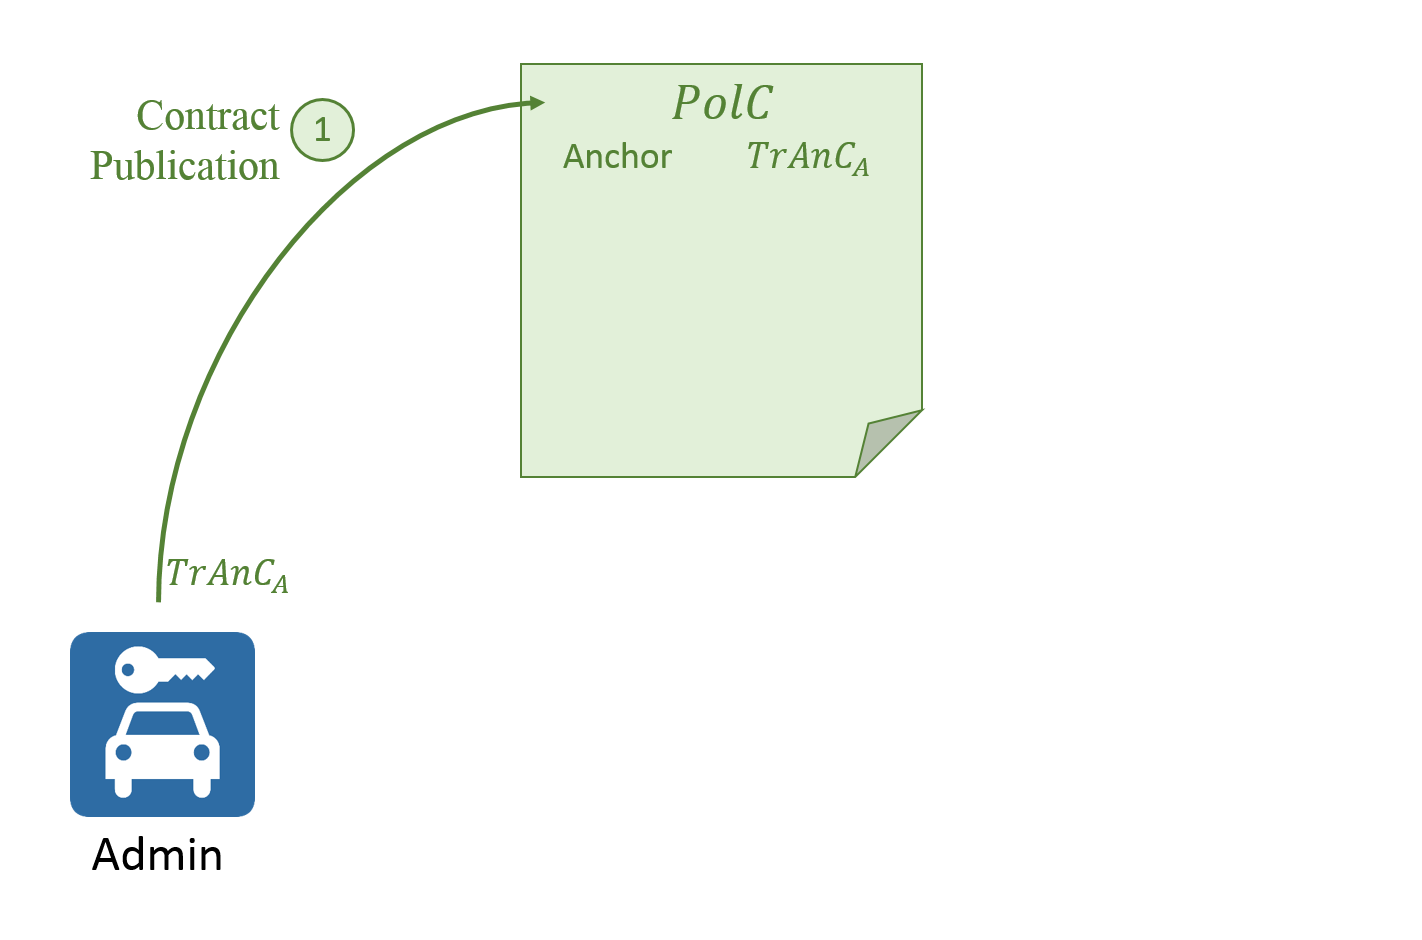
\includegraphics[scale=0.4]{Figures/PolC_1.png}}
        \only<2>{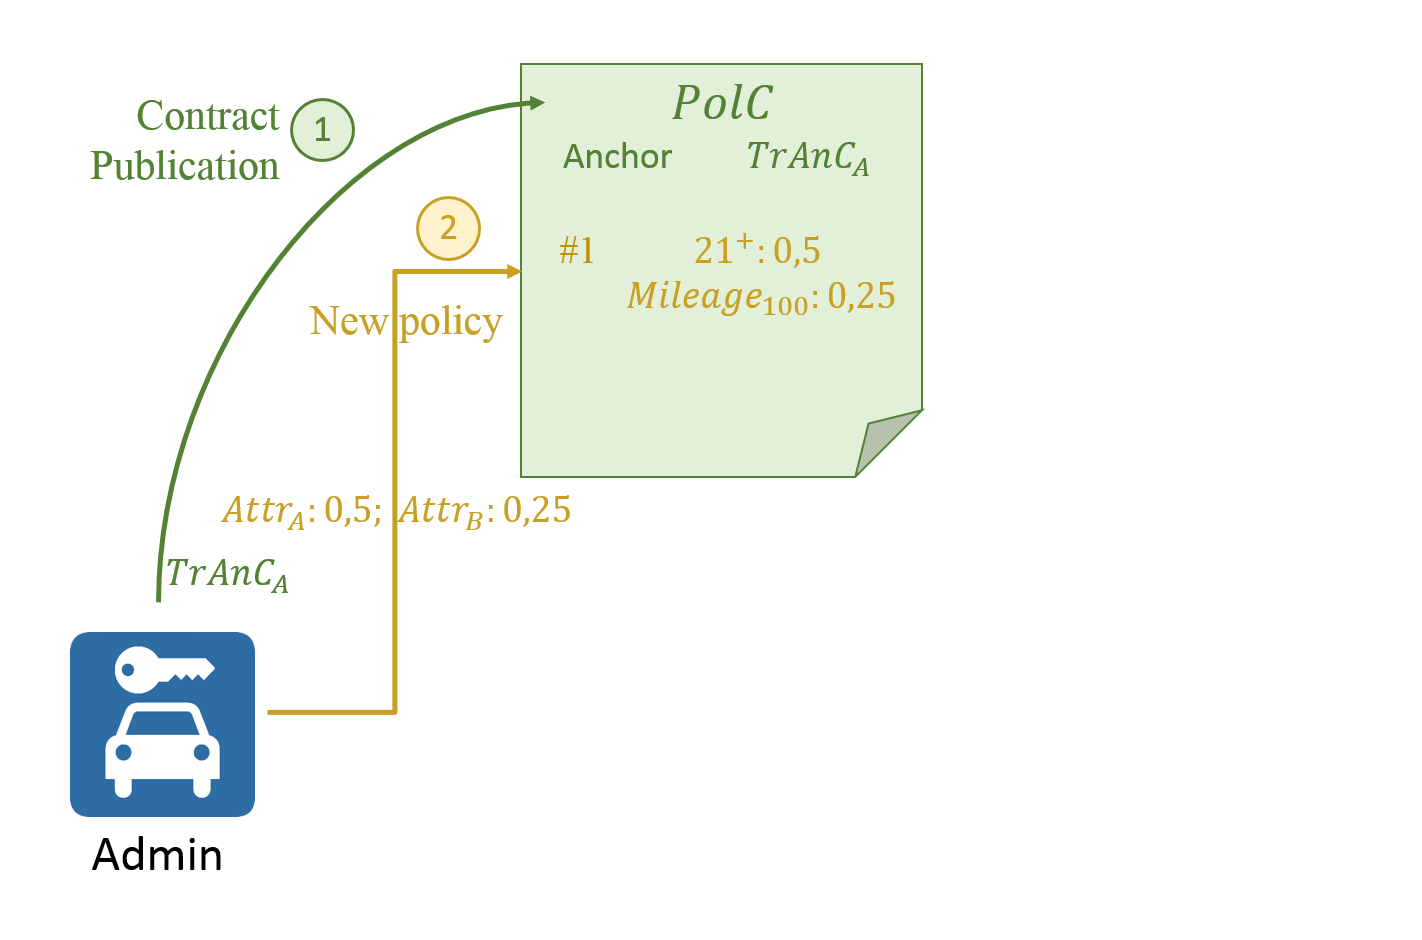
\includegraphics[scale=0.4]{Figures/PolC_2.png}}        
        \only<3>{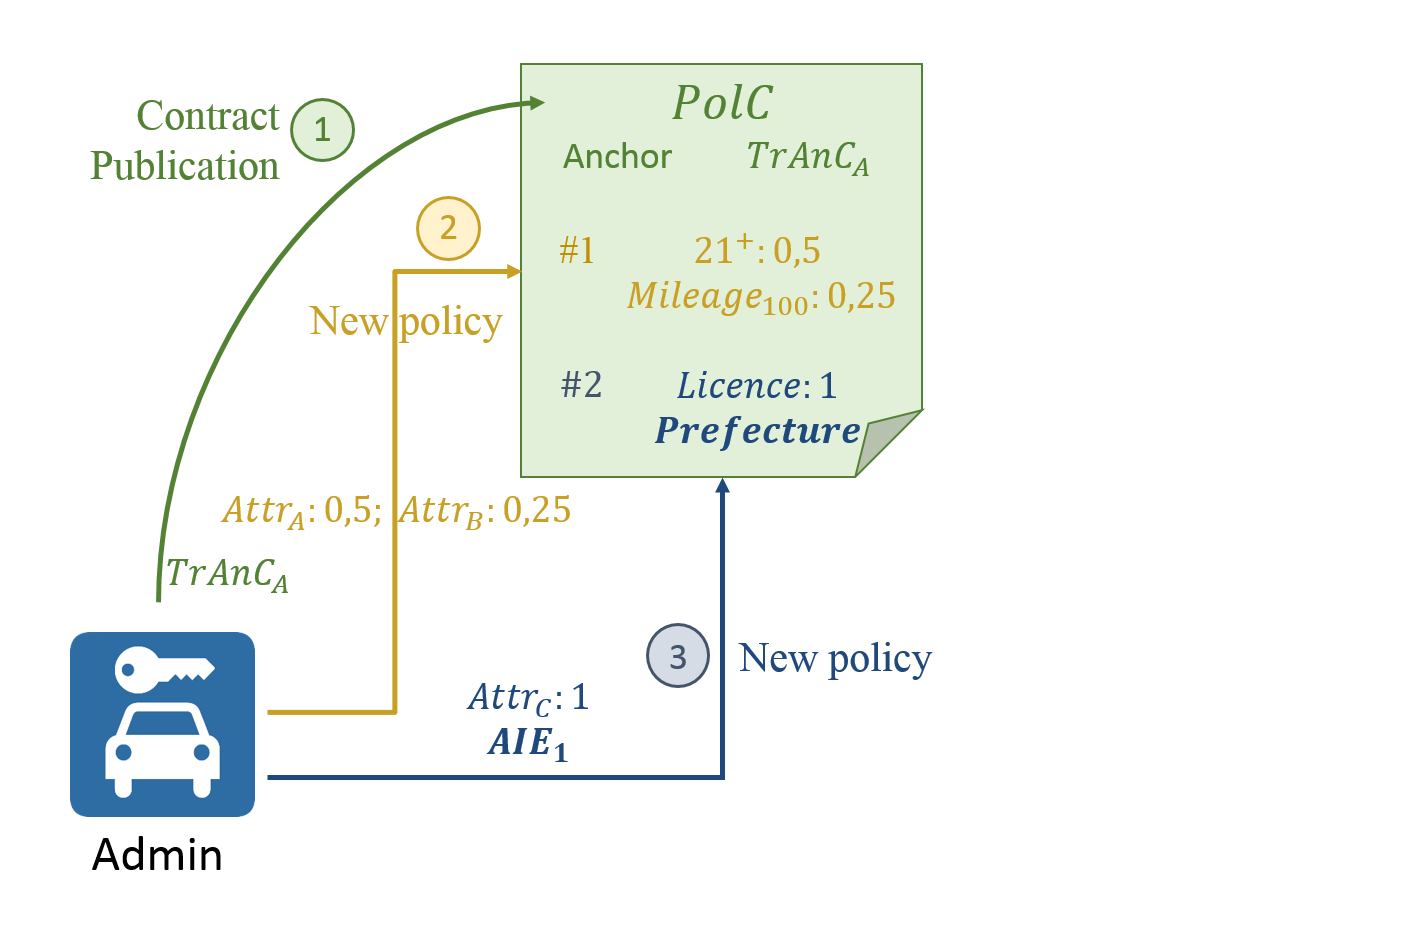
\includegraphics[scale=0.4]{Figures/PolC_3.png}}
        \only<4>{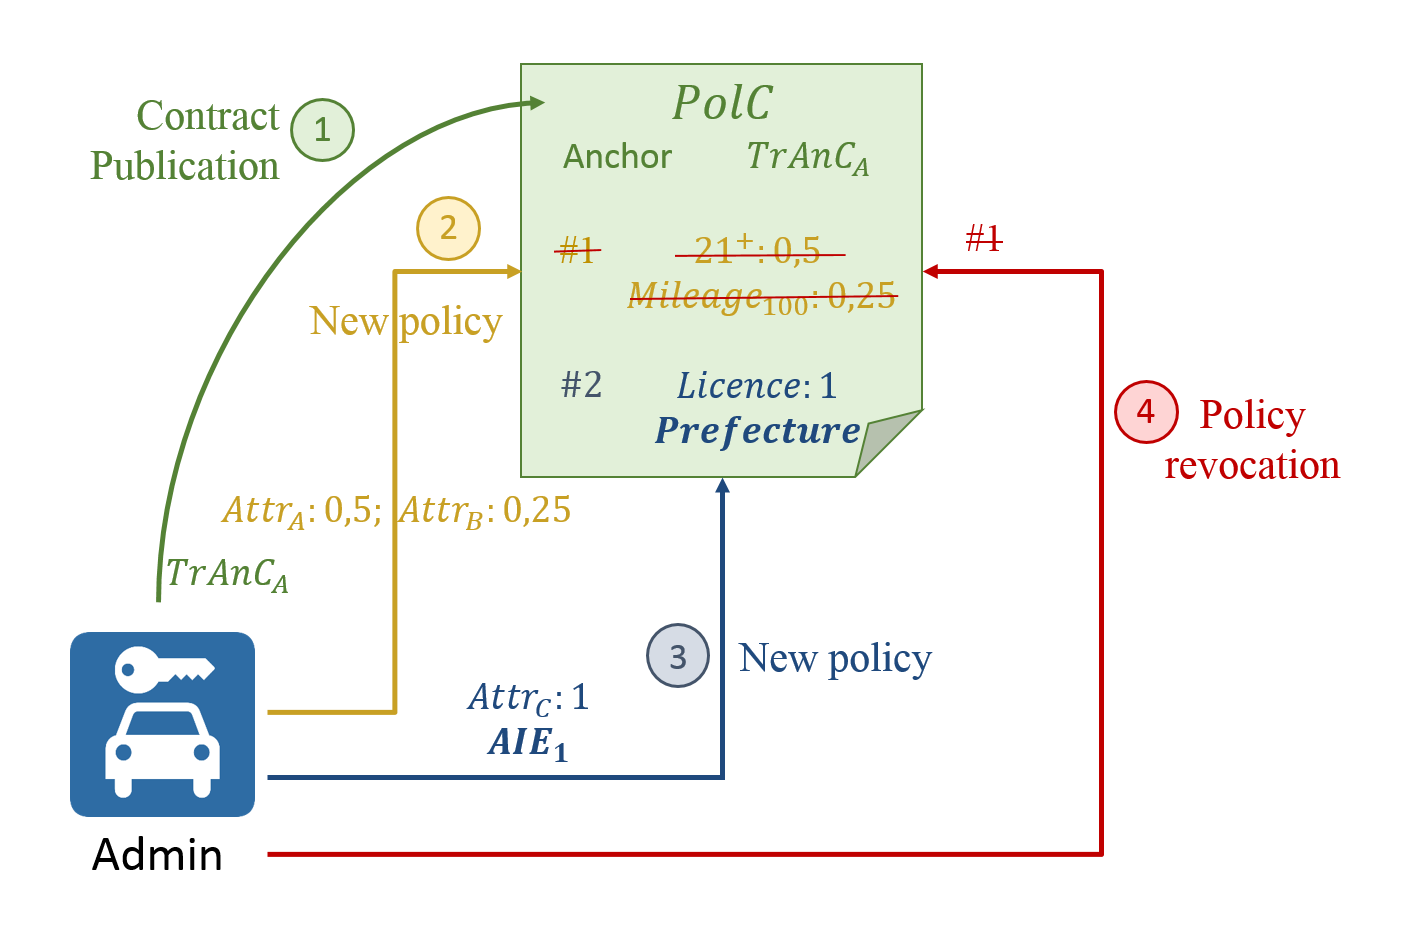
\includegraphics[scale=0.4]{Figures/PolC_4.png}}
    \end{center}
\end{frame}

% * * * * * * NEW FRAME * * * * * * %
\begin{frame}{Policy Service: Dispatch Contract (DisC)}
    \begin{center}
        \only<1>{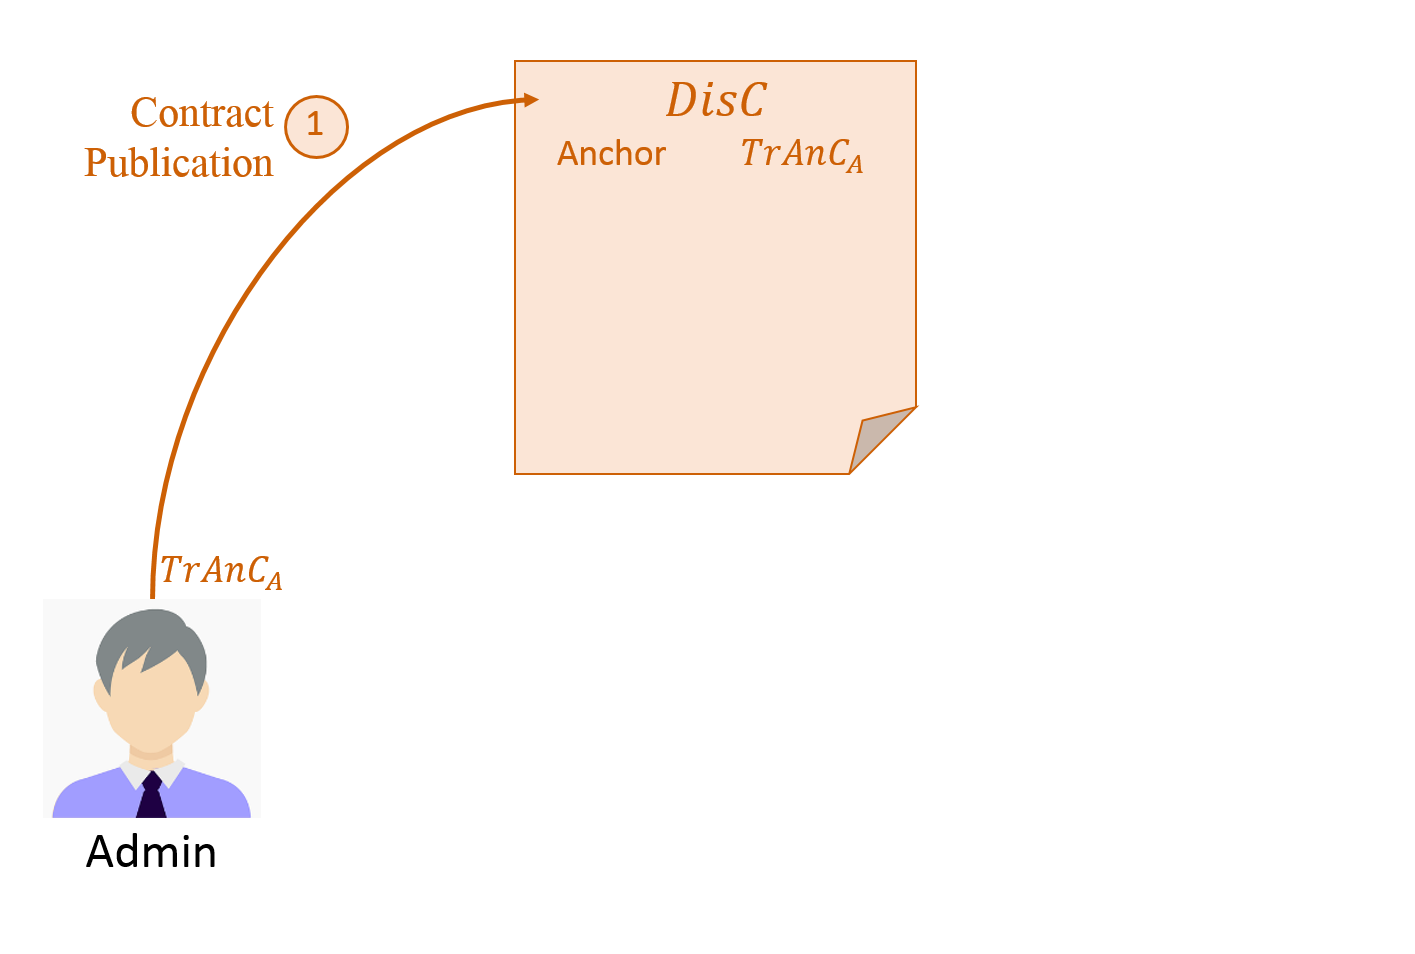
\includegraphics[scale=0.4]{Figures/DisC_1.png}}
        \only<2>{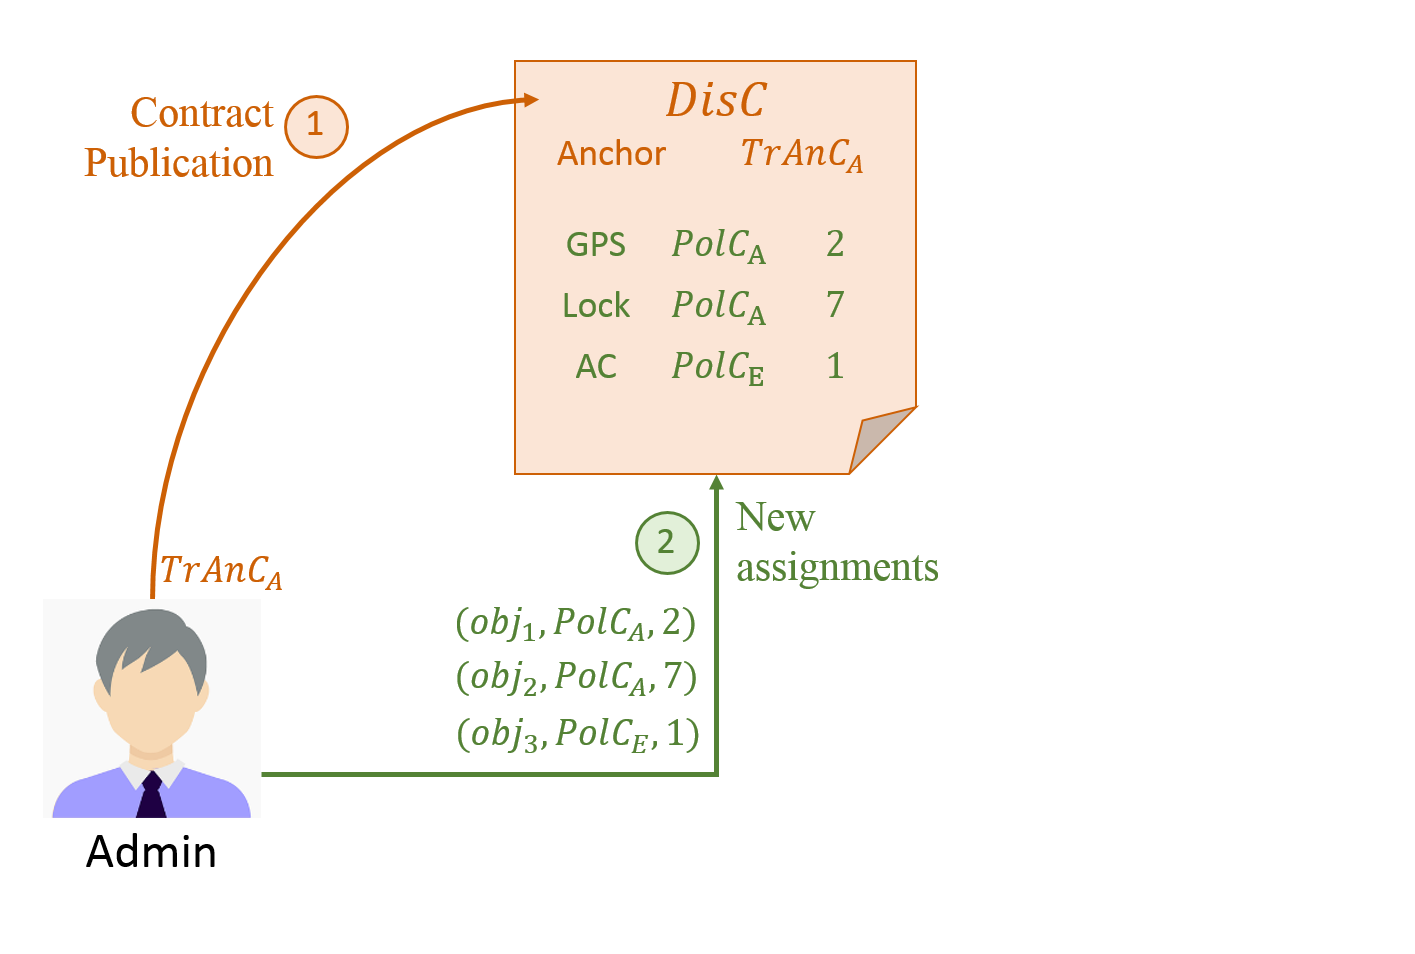
\includegraphics[scale=0.4]{Figures/DisC_2.png}}        
        \only<3>{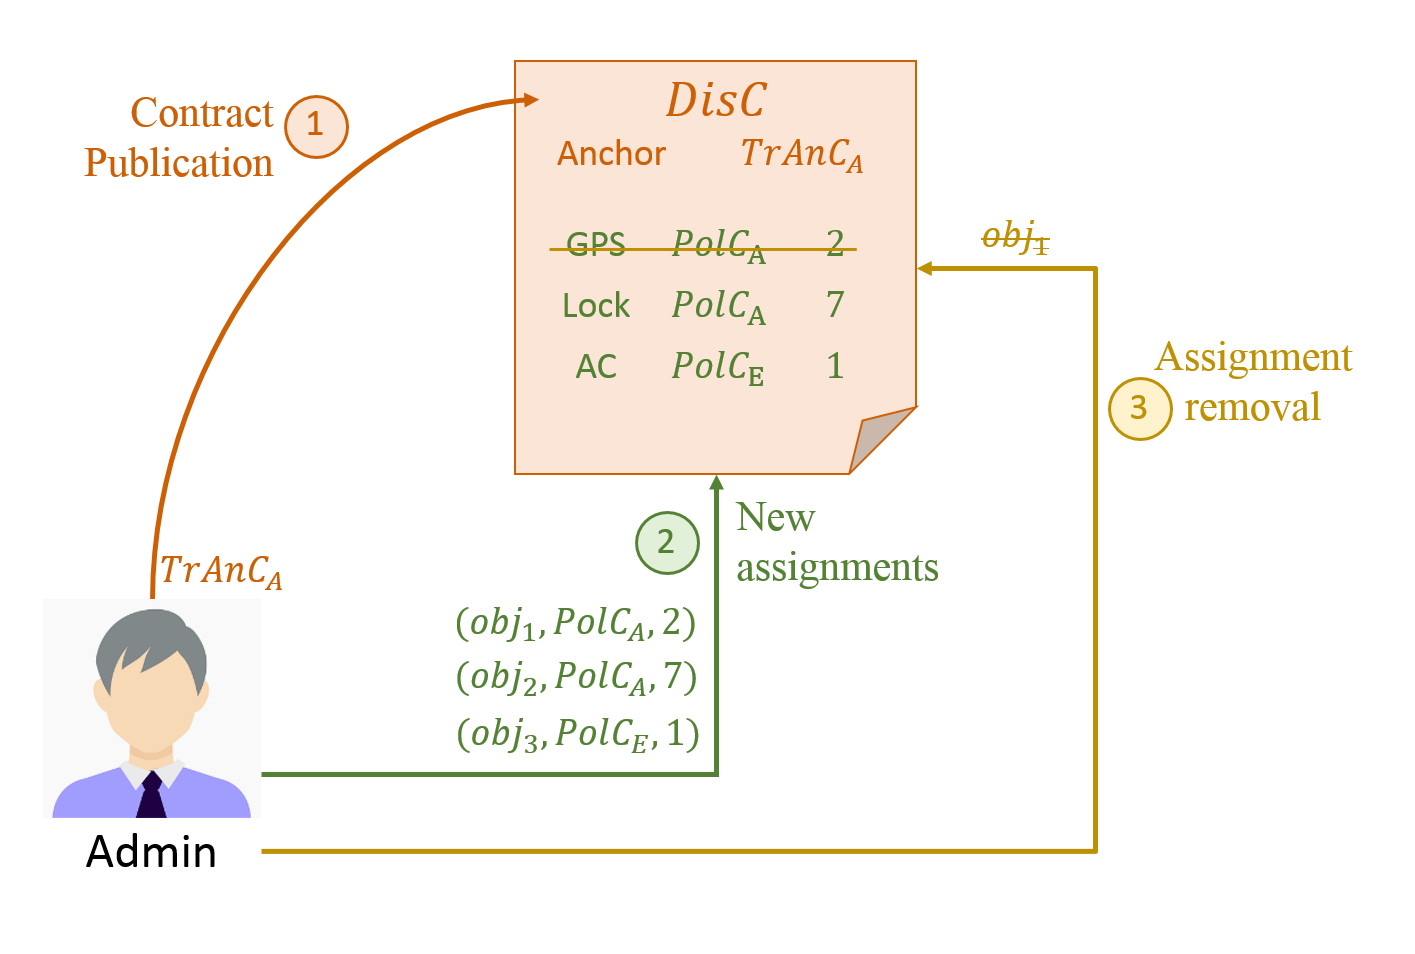
\includegraphics[scale=0.4]{Figures/DisC_3.png}}
    \end{center}
\end{frame}

% * * * * * * NEW FRAME * * * * * * %
\begin{frame}{Attribute Service}
    \begin{center}
        \only<1>{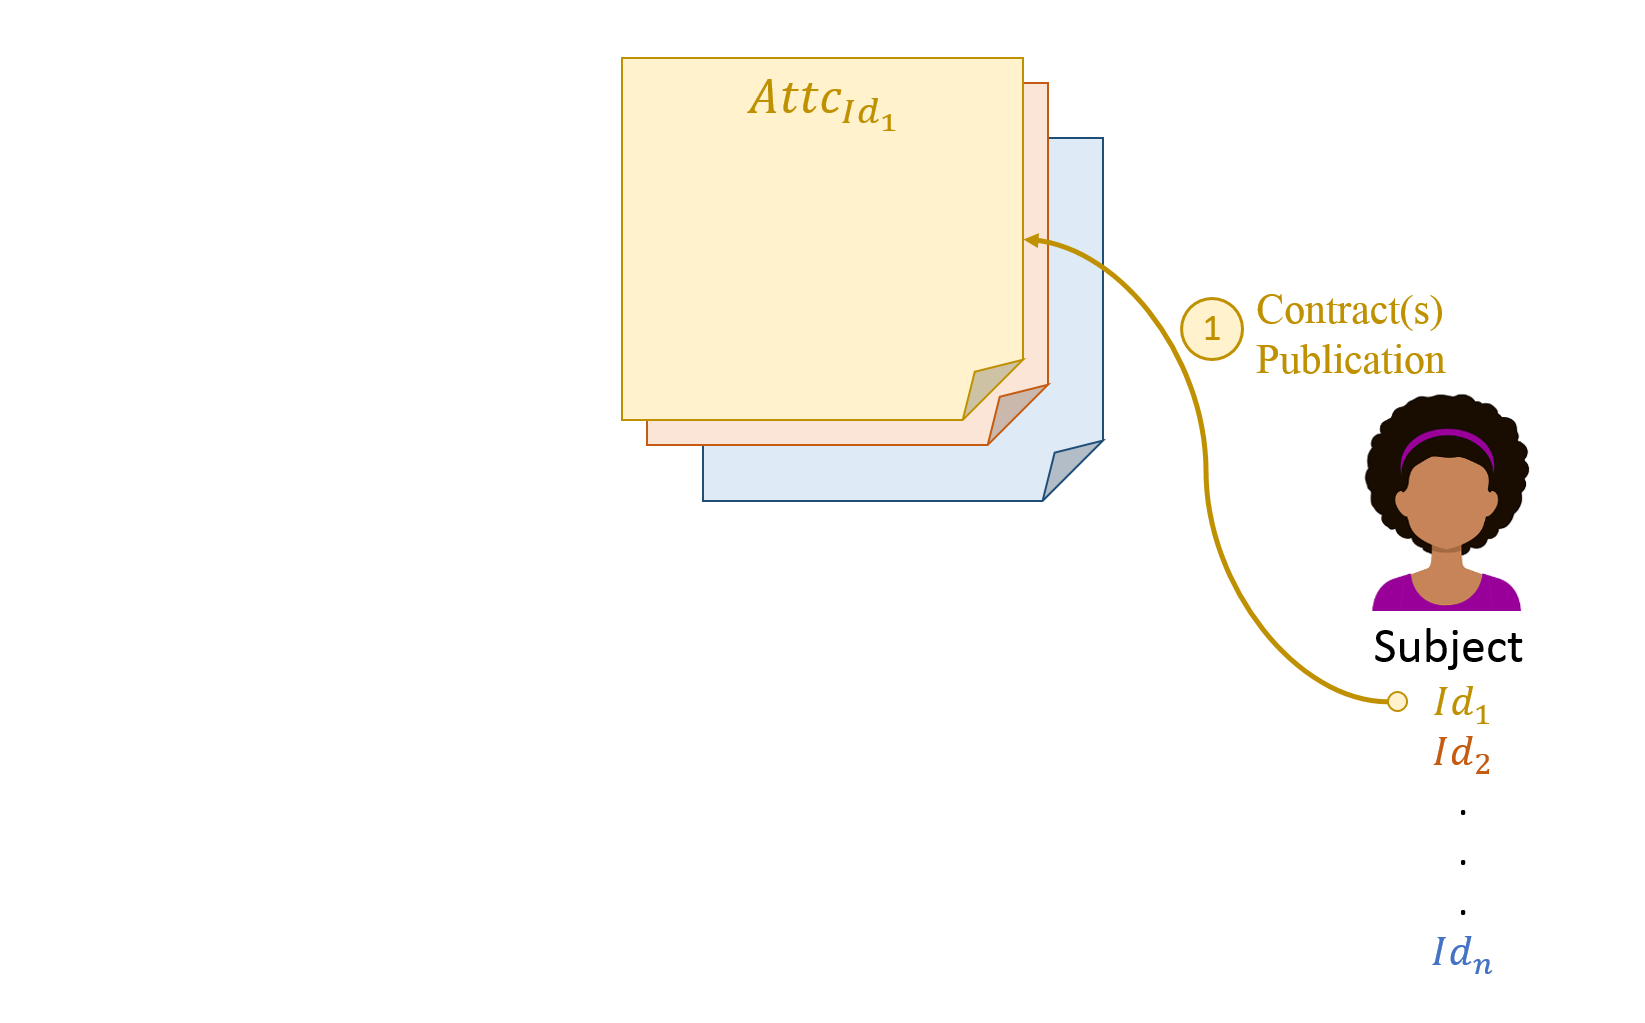
\includegraphics[scale=0.4]{Figures/AttC_1.png}}
        \only<2>{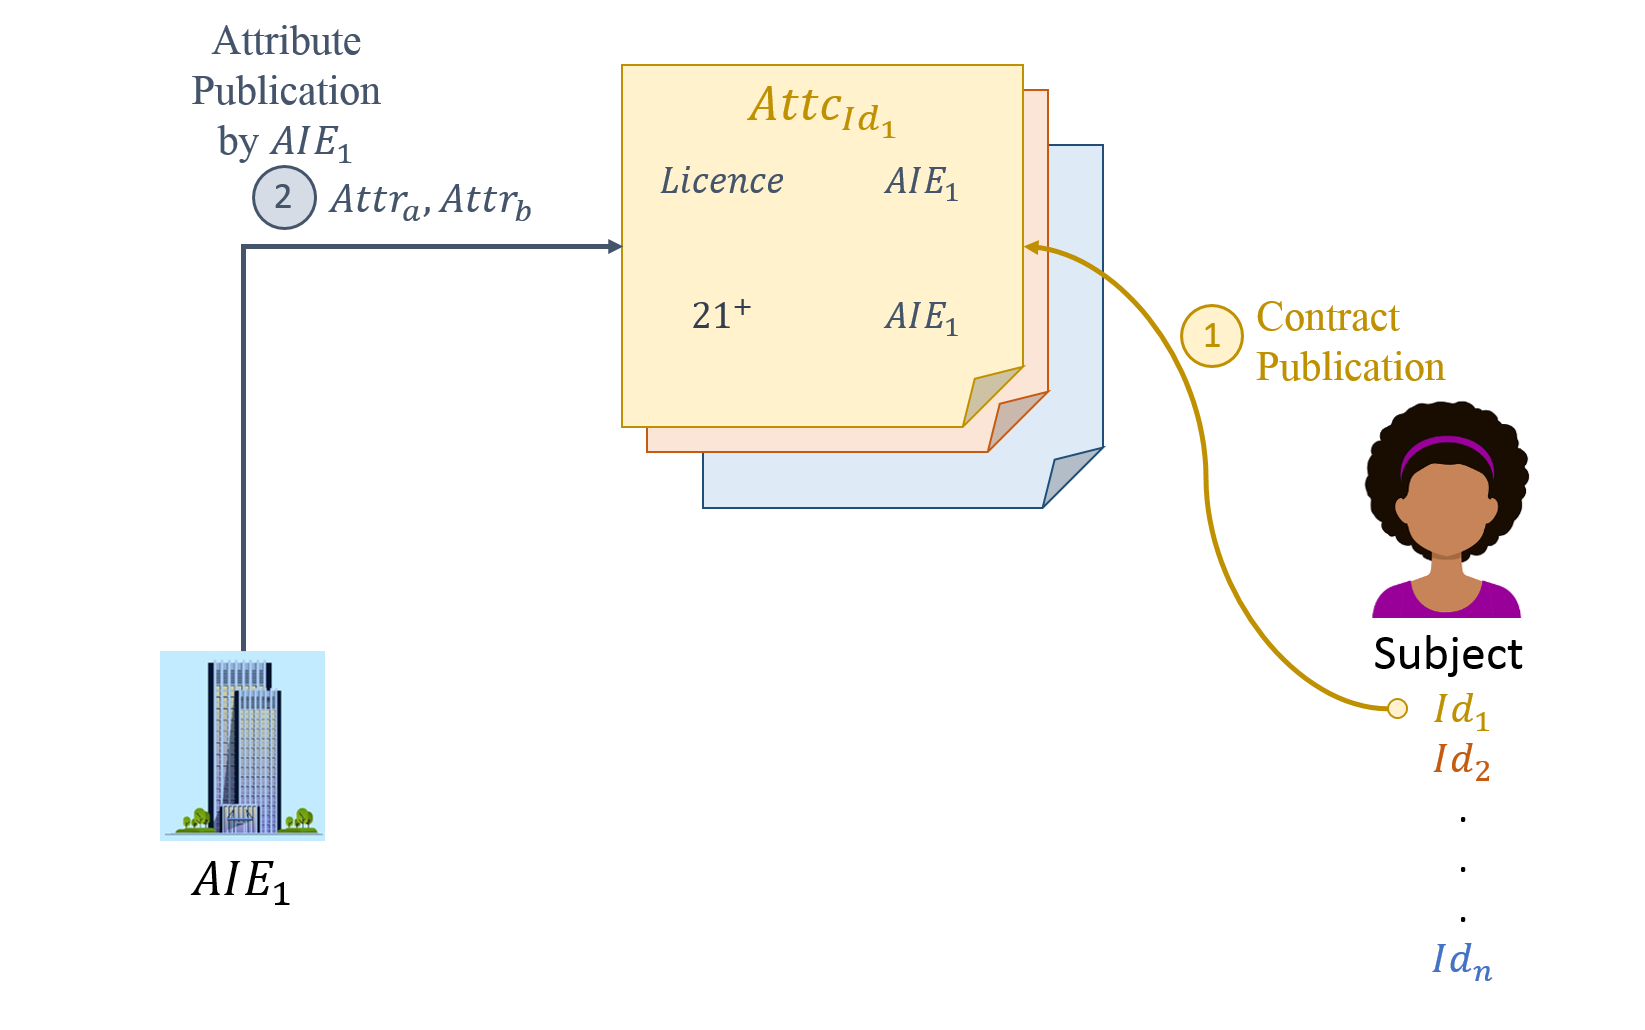
\includegraphics[scale=0.4]{Figures/AttC_2.png}}        
        \only<3>{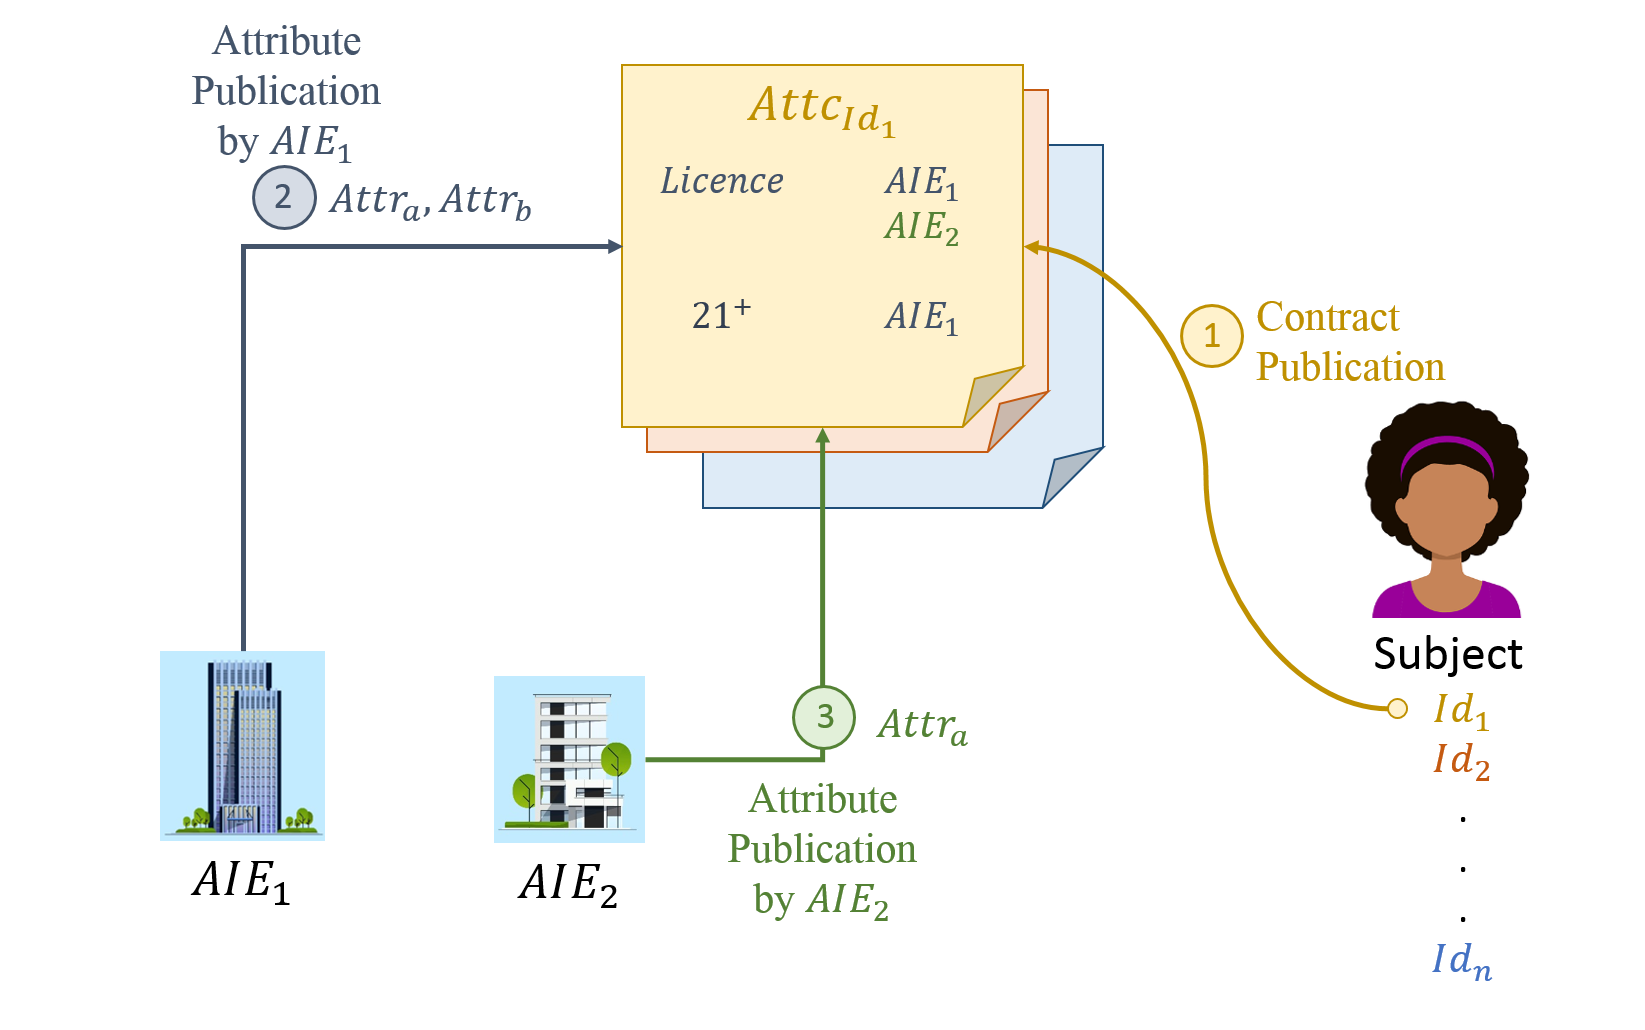
\includegraphics[scale=0.4]{Figures/AttC_3.png}}
        \only<4>{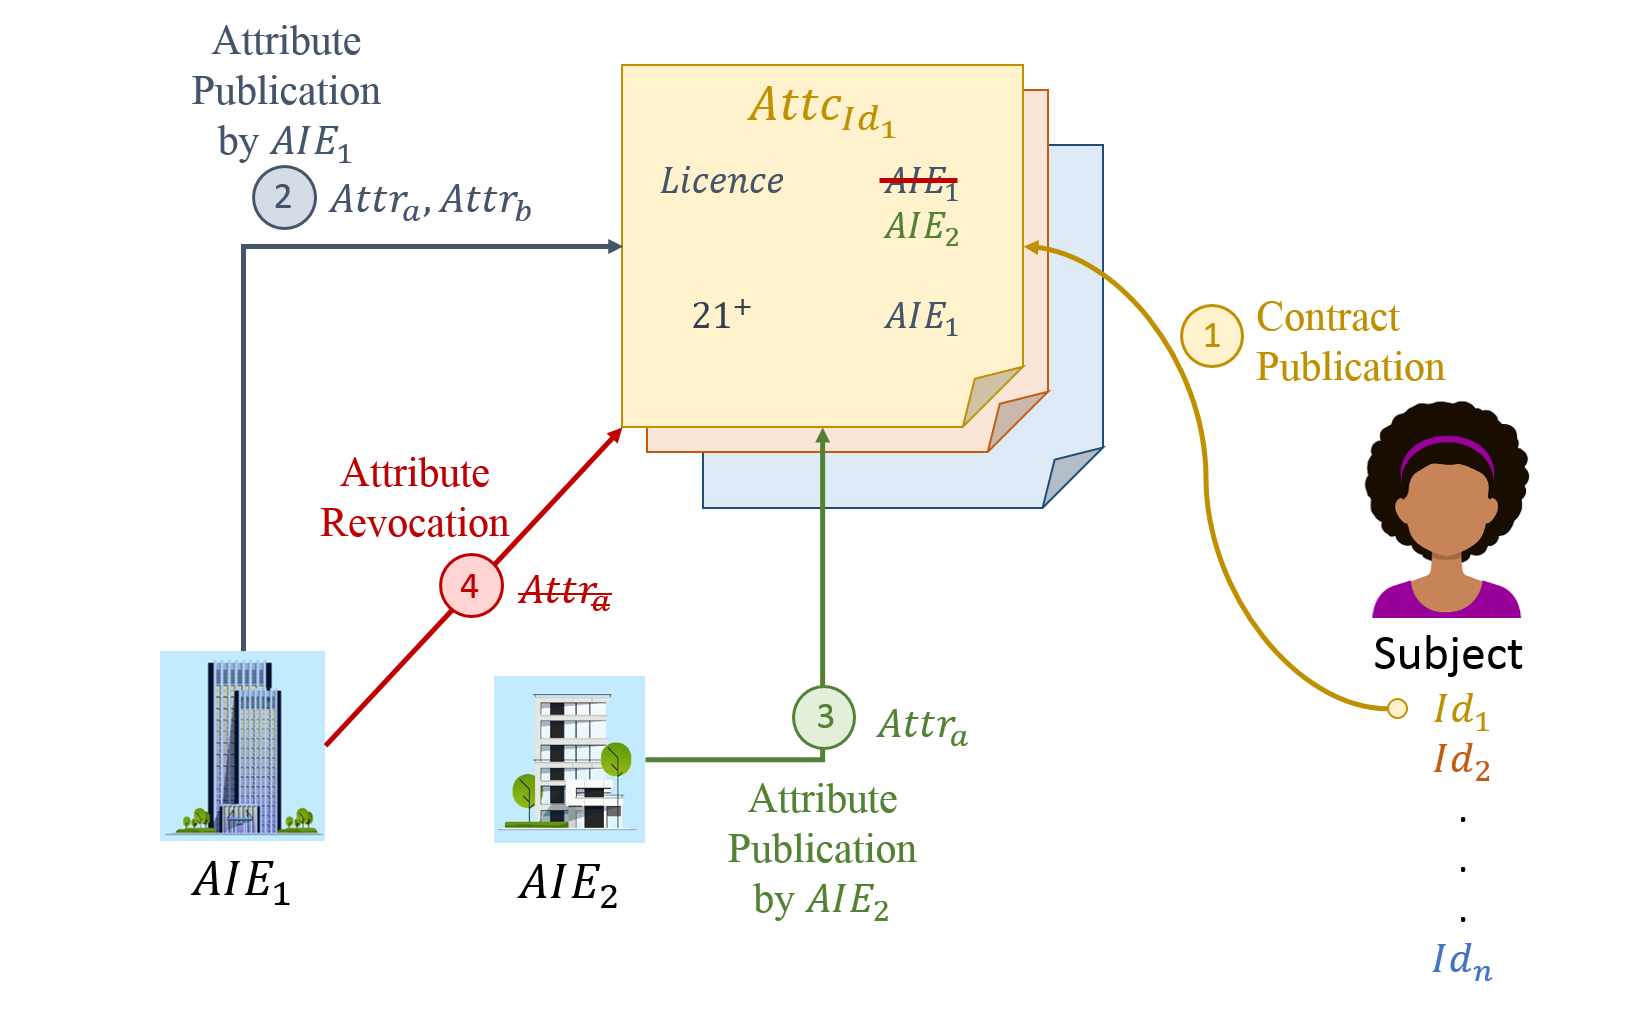
\includegraphics[scale=0.4]{Figures/AttC_4.png}}
    \end{center}
\end{frame}

\subsection{Access control}

% * * * * * * NEW FRAME * * * * * * %
\begin{frame}{Access control overview}
    \begin{center}
        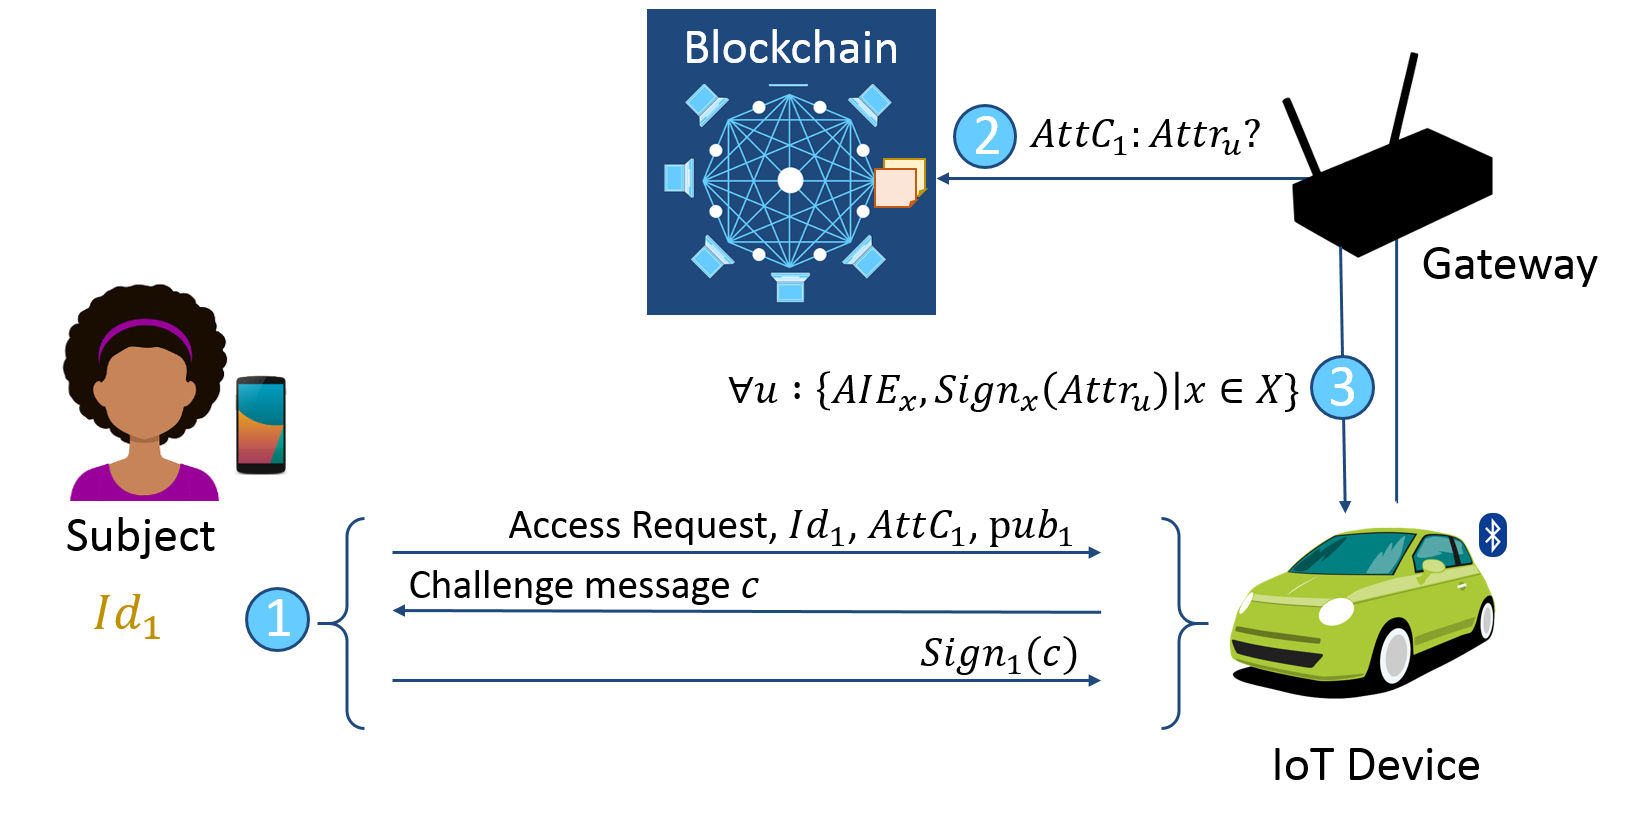
\includegraphics[scale=0.42]{Figures/MAAC-B_AC.png}
    \end{center}
\end{frame}

% * * * * * * NEW FRAME * * * * * * %
\begin{frame}{Trust level computation}
For $Attr_u$ and the corresponding endorsement set $End_u$:
    \begin{itemize}
        \item \emph{if $End_u = \emptyset$} 
        $$TL_u = 0$$
        
        \item \emph{if $End_u$ contains a TE endorsement} 
        $$TL_u = 1$$
        
        \item \emph{otherwise}, given a reputation system $RS$  
        $$TL_u = F(End_u, RS)$$ 
    \end{itemize}
    
Examples of formulas for $F$ include:
    \begin{itemize}
        \item $Max_x(Rep_x)$, where $Rep_x$ is the reputation of $AIE_x$
        \item $Min_x(Rep_x)$
        \item Average reputation score
    \end{itemize}

\end{frame}

\subsection{Conclusion}

% * * * * * * NEW FRAME * * * * * * %
\begin{frame}{Circling back to the requirements}

    \begin{table}[ht]
    \centering
    \small{
        %\rowcolors{1}{lightgray}{}
        \begin{tabular}{|c|c|}
            \hline
            Resource efficiency & ? \\ \hline
            Actuator-compatible & \textcolor{ao(english)}{\ding{51}} \\ \hline
            Revocation (implicit) & \textcolor{red}{\ding{55}} \\ \hline
            Revocation (explicit) & \textcolor{ao(english)}{\ding{51}}\\ \hline
            Granularity & \textcolor{ao(english)}{\ding{51}} \\ \hline
            Context-awareness & Client-wise \\ \hline
            
            \hline
            Interoperability & \textcolor{ao(english)}{\ding{51}} \\ \hline
            Dynamic users & \textcolor{ao(english)}{\ding{51}} \\ \hline
            User-centric & \textcolor{ao(english)}{\ding{51}} \\ \hline
            Scalability & \textcolor{ao(english)}{\ding{51}} \\ \hline
            Ease of management & \textcolor{ao(english)}{\ding{51}} \\ \hline
            Local access & \textcolor{ao(english)}{\ding{51}} \\ \hline
            
            \hline
            Privacy & \textcolor{ao(english)}{\ding{51}} \\ \hline
            Usability & \textcolor{ao(english)}{\ding{51}} \\ \hline
            Auditability & Policy-wise \\ \hline
            Governance & \textcolor{ao(english)}{Multi-head} \\ \hline
        \end{tabular}
        }
    \end{table}
    
\end{frame}

% * * * * * * NEW FRAME * * * * * * %
\begin{frame}{MAAC-B: Summary}

Contributions:
    \begin{itemize}
        \item User-controlled identities
        \item Entity-independent attribute management system
        \item Flexible trust anchors
        \item Attribute evaluation process based on reputation
        \item Distributed and generic policy management system
    \end{itemize}

\bigskip

Validation methods:
    \begin{itemize}
        \item Informal security analysis
    \end{itemize}
\end{frame}

